\chapter{ Investigating Tracking Improvements}
\label{chap:tracking}

Todo:
\begin{itemize}
    \item Check all info wrt to  \href{https://pdg.lbl.gov/2018/reviews/rpp2018-rev-b-meson-prod-decay.pdf}{this PDG review}
\end{itemize}


\section{Overview}\label{sec:tracking overview}

\subsection{B Hadron Reconstruction}\label{sec:b reconstruction}

\subsubsection{B Hadron Decay Topology}\label{sec:b decay topolgy}

\bhadrons are quasi-stable bound states of quarks, where one of the quarks is a bottom quark ($b$ quark). The proper lifetimes $\tau$ of the various \bhadrons are similar and relatively long, with $\tau \sim 10^{-12}$s. This lifetime corresponds to a proper decay length $c \tau \sim 300 ~\mu$m. In the rest frame of the detector, the typical \bhadron travels a distance $d = \beta\gamma c \tau$ before decaying, where at high energies $\gamma \sim E_B/m_B$. For a 1 TeV \bhadron, this gives $d \sim 60$ mm - well beyond the radius of the first pixel layer (IBL) at 33 mm.
%   
\begin{figure}[!hb]
    \centering
    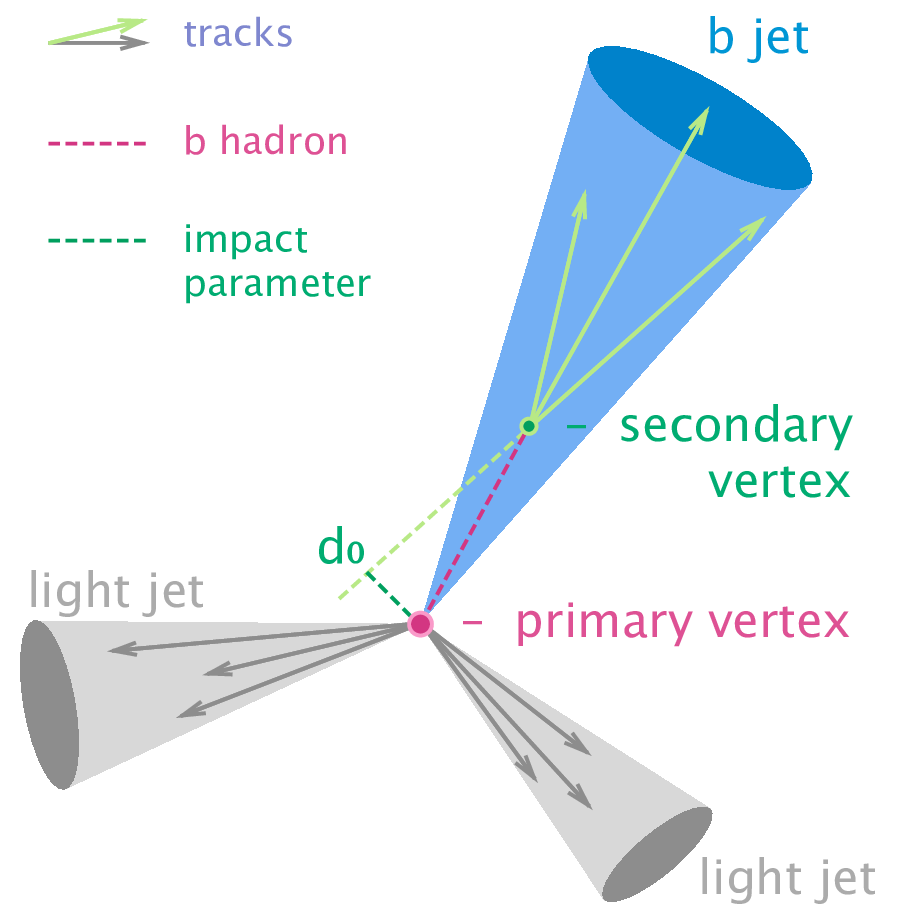
\includegraphics[width=0.25\textwidth]{chapters/3.tracking/figs/b-jet-diagram.png}
    \caption{Diagram of a typical \bjet (blue) which has been produced along with two light jets (grey). The \bhadron has travelled a significant distance from the primary interaction point (pink dot) before its decay. The large transverse impact parameter $d_0$ is a characteristic property of the trajectories of \bhadron decay products.}
    \label{fig:b-jet topology}
\end{figure}
%
At the LHC, $b$ quarks are generated in the hard scattering of proton-proton ($pp$) collisions. They quickly hadronize into a \bhadron, which is often initially in an excited state due to the high energies of the $pp$ collisions at the LHC ($\sqrt{s} = 13$ TeV). The hadronisation process is hard - around 70-80\% of the $b$ quark's momentum goes into the \bhadron, with the rest being radiated as other particles. The excited \bhadron will quickly fragment (i.e. de-excite) by radiating particles, which are prompt (they are formed closed to the primary vertex). These fragmentation particles have an increasing multiplicity and collimation to the \bhadron axis as the \pT of the \bhadron increases. The de-excited \bhadron subsequently weakly decays to on average $4$ or $5$ particles (the multiplicity of the decay products of the weak decay of the \bhadron is unaffected by increases in the \bhadron \pT.). 

Due to their lifetimes, energetic \bhadrons can travel a significant distance from the primary $pp$ interaction point before decaying to a spray of collimated stable particles. This signature is registered in the detector as a displaced jet. Due to the elements of the CKM matrix, \bhadrons decay with a high probability to D hadrons (which contain a $c$ quark), which also have significant lifetimes - this can lead to reconstructed tertiary vertices in the jet core. The typical features of a \bjet, and in particular the large track impact parameter $d_0$ which can result from displaced decays, are shown in \cref{fig:b-jet topology}.
%
\begin{figure}[!htbp]
    \centering
    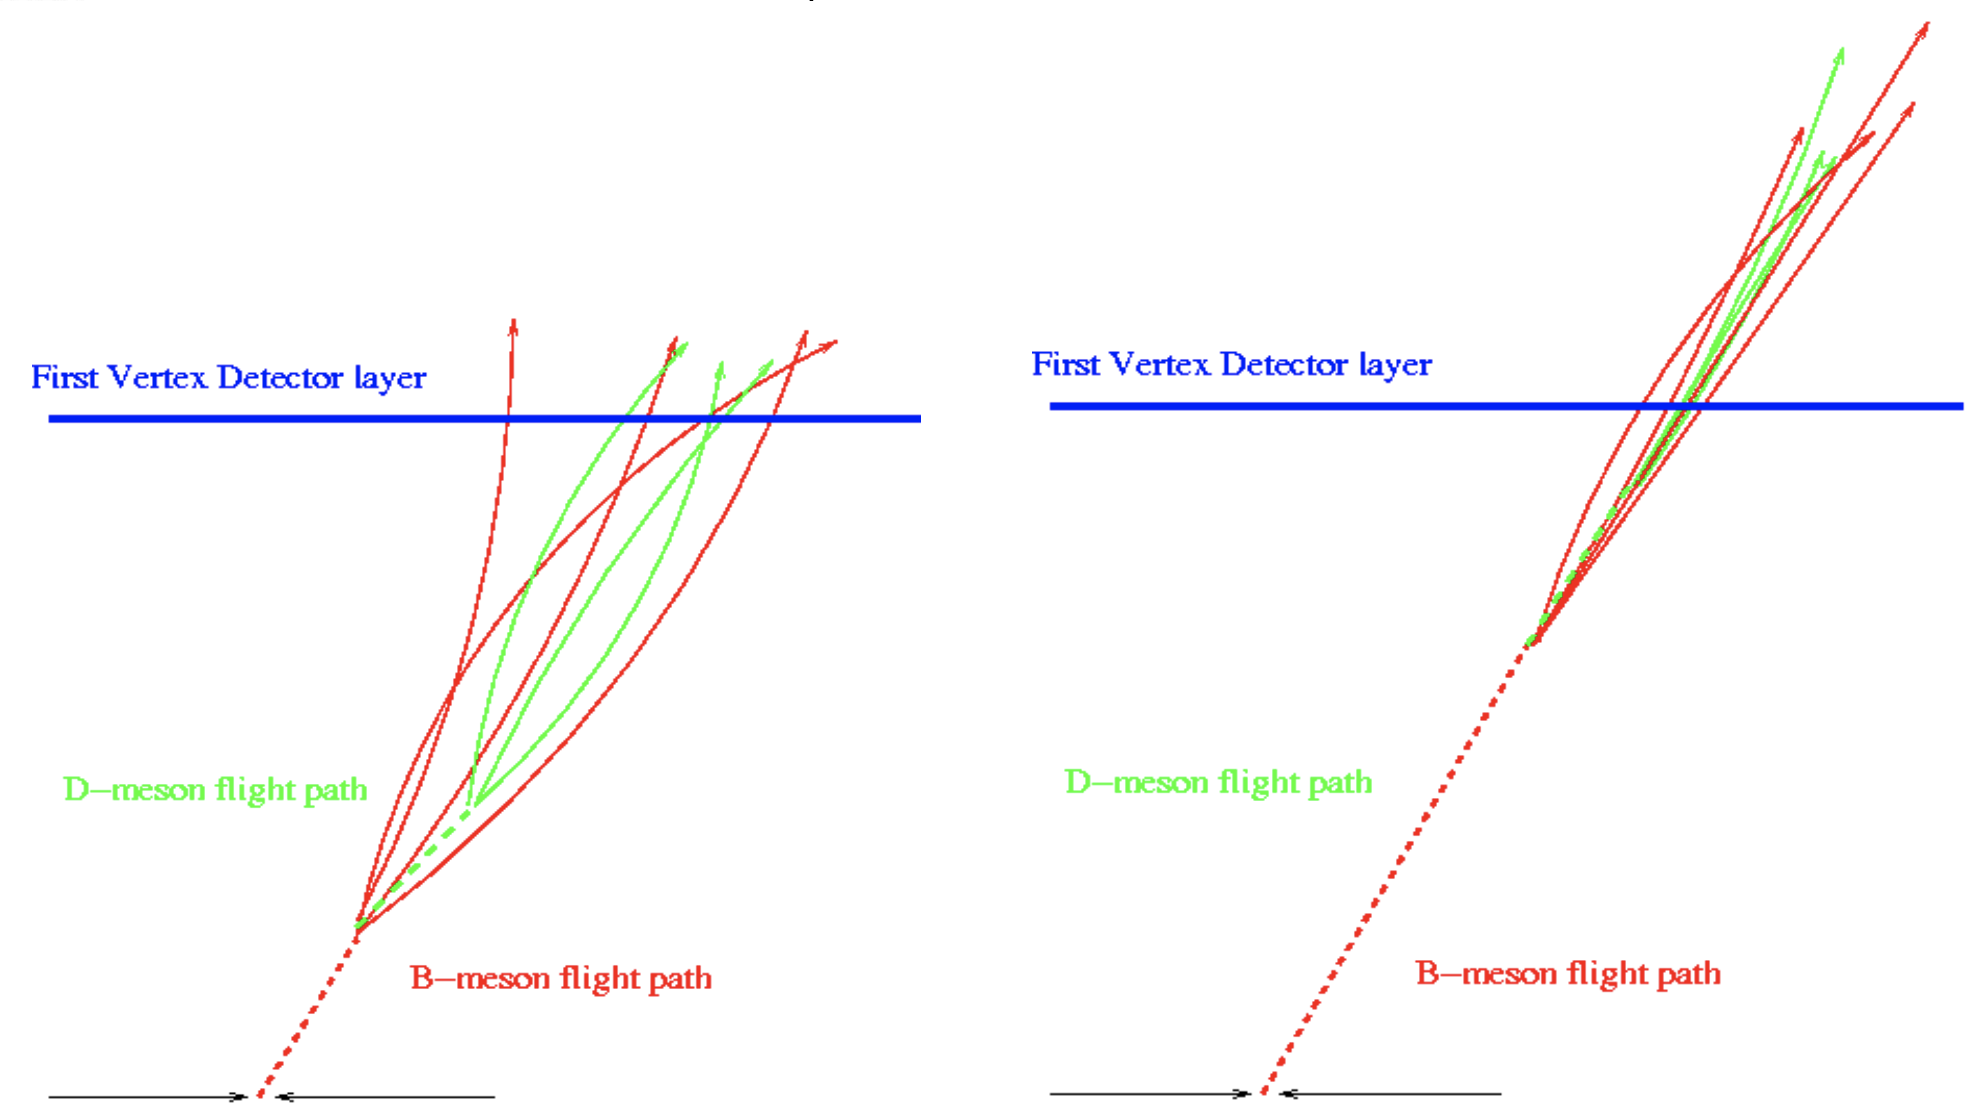
\includegraphics[width=0.7\textwidth]{chapters/3.tracking/figs/high-pt-b-tracks.png}
    \caption{As \bhadron $p_\text{T}$ increases, the time of flight of the B increases, so tracks will have less room to diverge before reaching detector elements. To compound the problem, the collimation of the tracks increases. The detector may then be unable to resolve individual tracks.}
    \label{fig:B hadron tracking problems}
\end{figure}
%
Many ATLAS analyses rely on a method of tagging jets instantiated by $b$ quarks and rejecting jets created from other quarks ($c$ and light flavours $u$, $d$, $s$). These ``\btagging'' algorithms work by discriminating against the unique signatures of \bjets discussed above. \btagging relies on the efficient and accurate reconstruction the tracks corresponding to the \bhadron decay products. These tracks are then used as inputs to vertex reconstruction algorithms and jet making algorithms.


\subsubsection{B Hadron Track Reconstruction Challenges}\label{sec:B track reco challenges}

A necessary requirement for successful jet \btagging is the efficient and accurate reconstruction of the charged particle trajectories in the jet. For high \pT jets (\pT $> 200$ GeV) this task becomes difficult due to a combination of effects. As the jet energy increases, the track multiplicity of the jet increases due to the presence of additional fragmentation tracks. Tracks in the jet also become increasingly collimated as their inherited transverse momentum increases. Together, these two effects lead to a very high density of charged particles in the jet core, making reconstruction difficult. At high energies, the increased decay length of B (and D) hadrons means that decay products have less of an opportunity to diverge before reaching the first tracking layers of the detector. If the decay takes place very close to a detector layer, or if the decays are sufficiently collimated, hits left by nearby particles may not be resolved individually, leading to merged clusters (shown in \cref{fig:B hadron tracking problems}). Shared hits generally predict bad tracks. As such, shared hits are heavily penalised during reconstruction (and in particular as part of ambiguity solving). However, in the core of high \pT \bjets, where decay particles are displaced from the primary vertex and are highly collimated, the density of particles is high enough that the probability of clusters being merged increases dramatically. The presence of merged clusters requires that the corresponding tracks share hits (if they are to be reconstructed successfully), which may end up impairing the successfully reconstruction of the track. Furthermore, decays may also take place inside the tracking detectors themselves, which can lead to missing or wrong innermost cluster assignment. The combination of effects described above makes reconstructing tracks in the core of high \pT \bjets particularly challenging.


%
\begin{figure}[!htbp]
    \centering
    \begin{subfigure}{.5\textwidth}
      \centering
      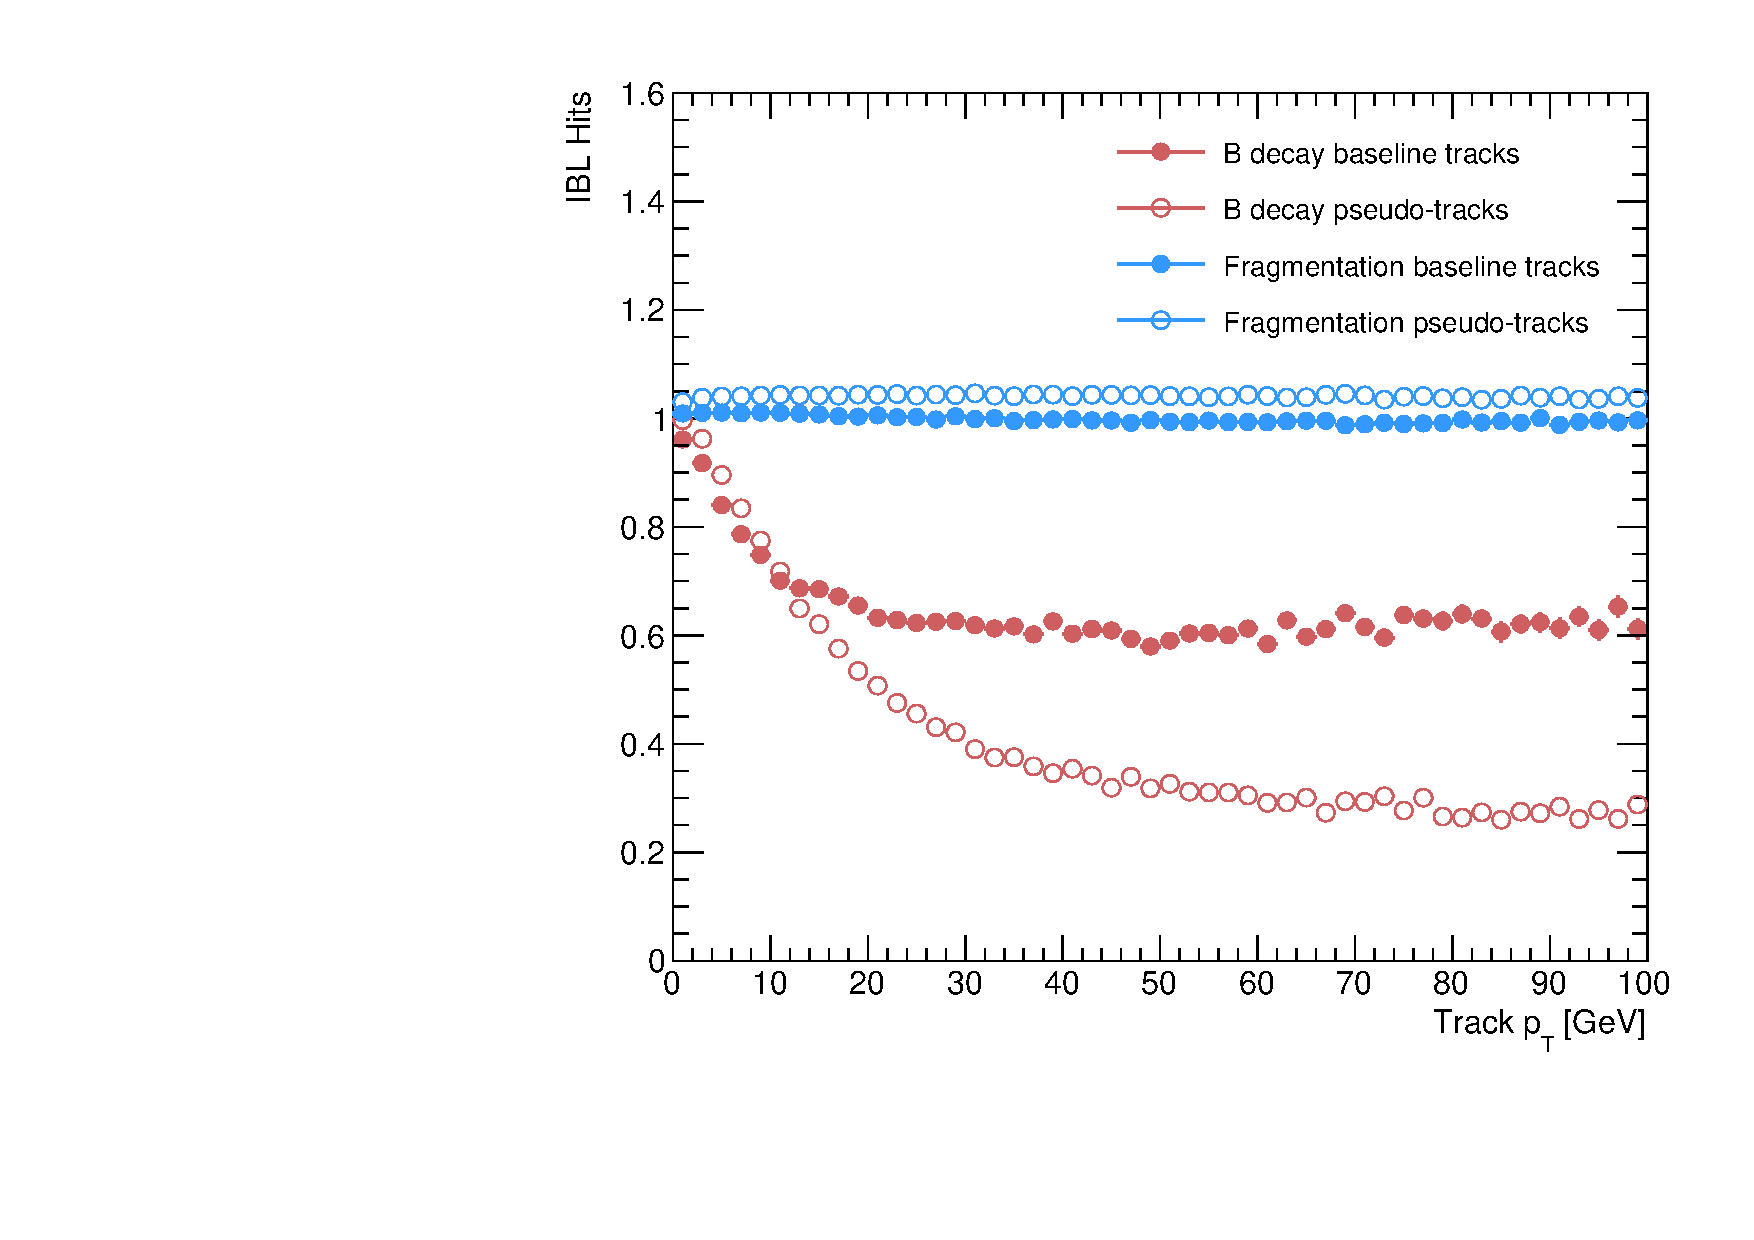
\includegraphics[width=\textwidth]{chapters/3.tracking/figs/overlay_po_nHitsOnIBL_From_B_pT.pdf}
      \caption{}
      \label{fig:n hits on ibl}
    \end{subfigure}%
    \begin{subfigure}{.5\textwidth}
      \centering
      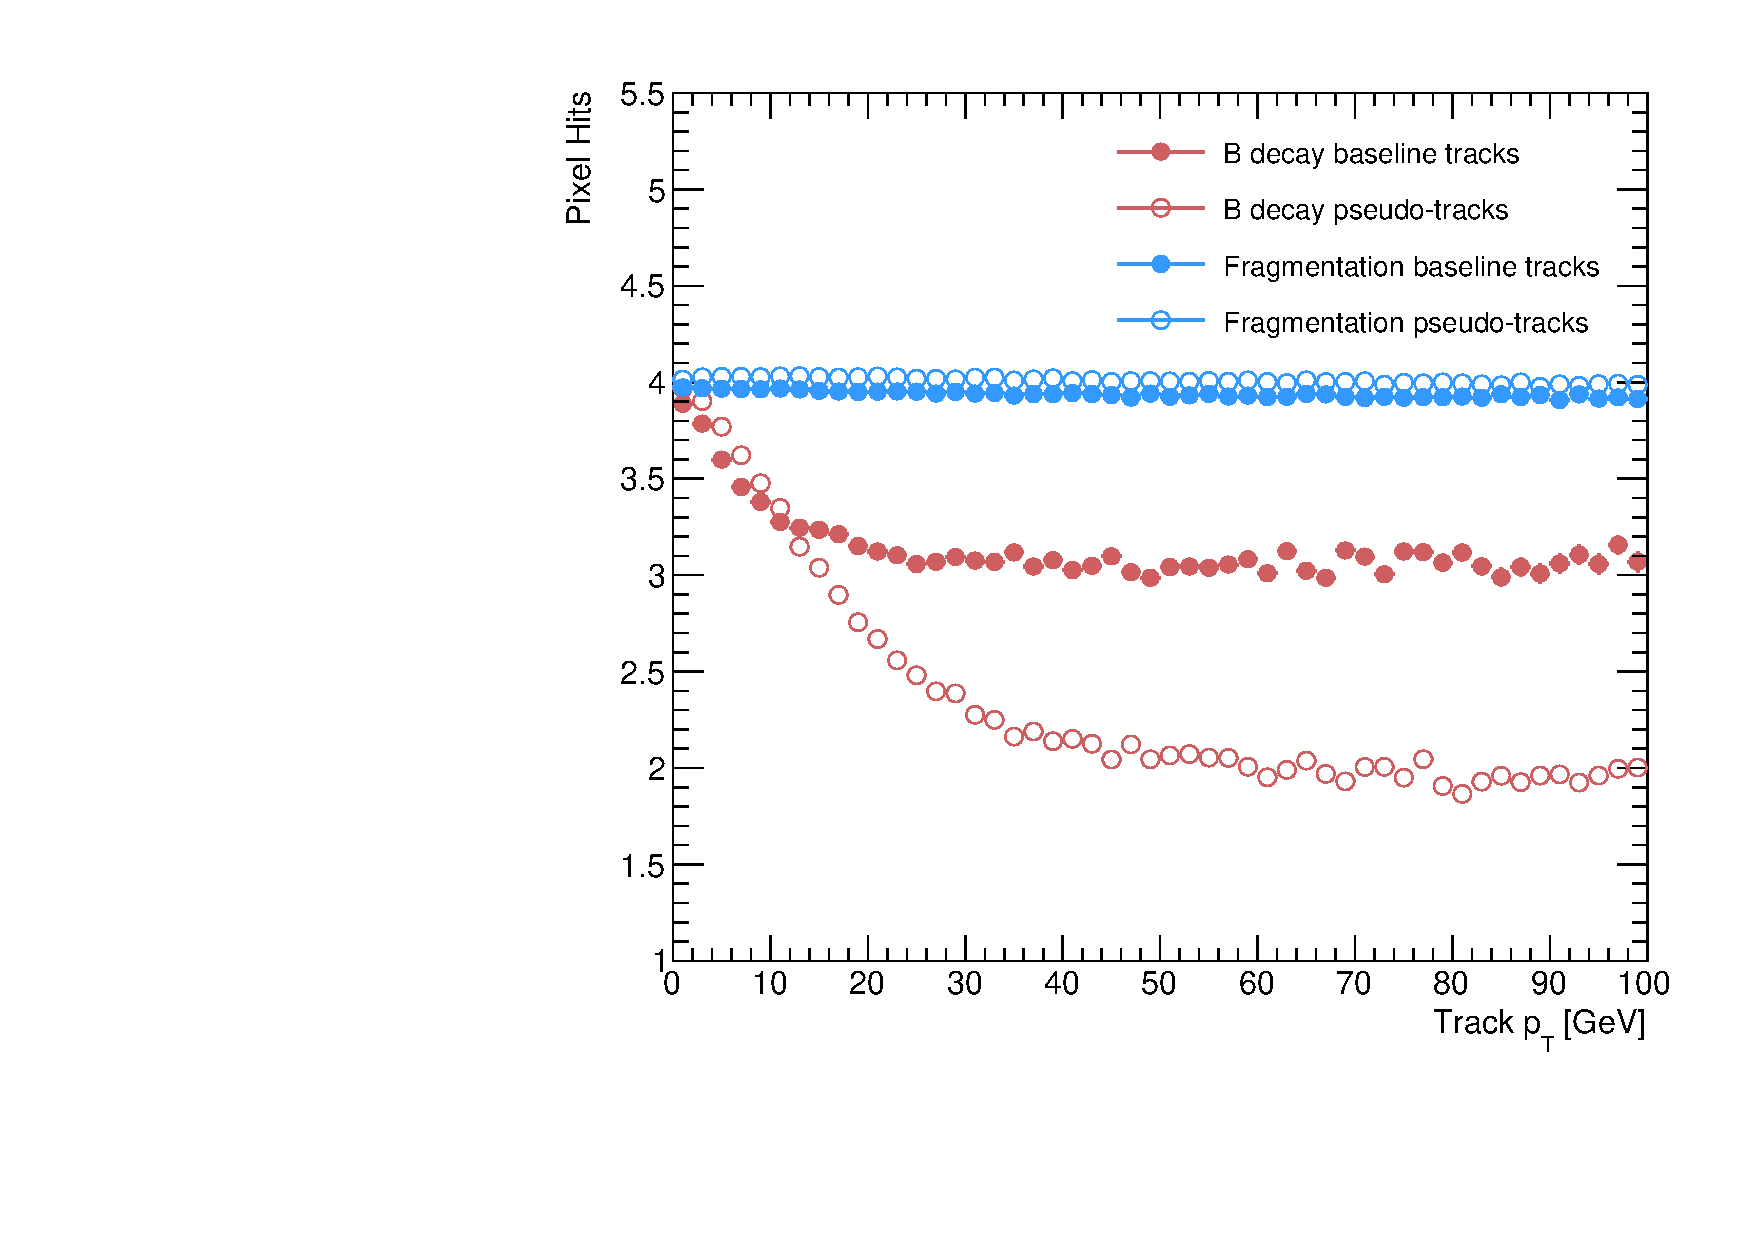
\includegraphics[width=\textwidth]{chapters/3.tracking/figs/overlay_po_nHitsOnPix_From_B_pT.pdf}
      \caption{}
      \label{fig:n hits on pix}
    \end{subfigure}
    \caption{Hit multiplicities on the IBL (\cref{fig:n hits on ibl}) and the all pixel layers (\cref{fig:n hits on pix}) as a function of the transverse momentum \pT of the reconstructed track. Tracks from the weak decay of the \bhadron are shown in red, while fragmentation tracks (which are prompt) are in blue. For each of these, standard tracks and pseudo-tracks are plotted. Hit multiplicities on the pseudo-tracks at high $p_\text{T}$ due to the increased flight of the \bhadron. The baseline tracks have more hits than the pseudo-tracks, indicating that they are being incorrectly assigned additional hits.}
    \label{fig:total hits on pix bs, frag}
\end{figure}
%







%
\begin{figure}[!htbp]
    \centering
    %\includegraphics[width=\textwidth]{res/figs/results/tracking/b-reco-efficiency.png}
    \vspace{0.05em}
    \caption{Track reconstruction efficiency from \bhadron decay products for baseline ATLAS tracking (black), Bcut+Refit procedures applied (green), pseudo-tracking (blue), and for tracking where the ambiguity solver has been manually removed (orange).}
    %The relatively high reconstruction efficiency at the stage of the track candidates (i.e. before ambiguity solving) indicates that the efficiency loss is driven by the ambiguity solver.
    \label{fig:reconstruction efficiency from B}
\end{figure}

\begin{figure}[!htbp]
    \centering
    %\includegraphics[width=\textwidth]{res/figs/results/tracking/po_nHitsOnPix_From_B_DL.pdf}
    \vspace{0.05em}
    \caption{The total number of pixel hits on tracks from \bhadron decays as a function of the production radius of the decay product. An excess of hits is assigned to the standard tracks in comparison to the ideal pseudo-tracks.}
    \label{fig:total hits on pix from b}
    \label{fig:misc}
\end{figure}
%

Concretely, then, the issues relating to high \pT \bhadron tracking can be factorised into two parts. The first part is a drop in track reconstruction efficiency. As mentioned, tracks originating from high energy \bhadron decay products can have a high rate of shared hits due to the number of particles present in a high \pT \bjet and their relative collimation. Additionally, tracks may be missing hits on the inner layers of the detector. This occurs primarily when the decay \bhadron decays inside the detector. These features of can make it difficult for B decay tracks to meet the ambiguity solver's stringent track quality requirements. As a result, many B decay tracks are rejected in the ambiguity solving stage, leading to a severe drop in tracking reconstruction efficiency. This is shown by the severe decrease in reconstruction efficiency visible when comparing baseline tracking with the ideal pseudo-tracks in \cref{fig:reconstruction efficiency from B}. This situation presents a problem: relaxing cuts on shared hits significantly degrades the ambiguity solver's power to reject bad tracks. However for \bhadron decay tracks it seems these same restrictions on shared hits are seriously impairing the reconstruction efficiency of good tracks. The second part of the problem is that, due to the high density of clusters available for assignment in the vicinity of the typical high energy \bhadron decay track, and also given the strong positive bias of the ambiguity solver towards those tracks with precise pixel measurements (especially the innermost IBL measurement), many \bhadron decay tracks are assigned incorrect inner layer hits. This is only a problem for those decay products which were produced inside the pixel detector as a result of a long-flying \bhadron, and so do not have a correct hit available for assignment (evidenced in \cref{fig:refit optimisation results sub2}). The incorrect hits may skew the parameters of the track, which can in turn mislead \btagging algorithms. In particular, \btagging algorithms rely heavily on the transverse impact parameter significance $d_0/\sigma(d_0)$ of the track. The quality of this measurement is expected to be adversely affected by wrong inner-layer hits on the track. This combination of reduced reconstruction efficiency and incorrectly assigned hits is thought to be the cause of the observed drop in \btagging efficiency at high energies , although it is not clear which effect may dominate.


\subsection{Pseudotracks and Ideal Tracks}\label{sec:pseudo ideal tracking}

Pseudotracking and ideal tracking are used as benchmarks of the best tracking possible given the ATLAS detector. Both pseudotracks and ideal tracks are constructed using truth information to group combinations of hits that have been left by the same truth particle. As a result, hit-to-track association and track reconstruction efficiency are both ideal (given the ATLAS detector). Ideal tracks represent a yet more idealised tracking scenario by correcting the cluster positions based on truth information, and smearing the cluster position based on the detector resolution.

When pseudotracking is run alongside standard tracking, those clusters which are shared on the reconstructed tracks run through the cluster splitting machinery. If a cluster is found to be compatible with being split, its definition is changed, and the pseudotracks use this definition too. As a result, pseudotracks can have split clusters.


\section{Track Labelling}\label{sec:track labelling}

\subsection{B Tracks}\label{sec:B track labelling}
\subsection{Fake Tracks}\label{sec:fake track labelling}

\section{Investigating Improvements for High \texorpdfstring{\pT}{pT} B Tracking}\label{sec:investigating tracking improvements}

An investigation into

\subsection{TrackAnalysis Package}\label{sec:track analysis package}


\subsection{Looser Track Cuts \& Track Refit Procedure}\label{sec:bcut and refit}

A solution for the problem of wrong inner-layer hits on $B$ tracks had previously previously been developed. This solution selects tracks which pass a $b$-jet Region of Interest (ROI) selection, and then removes the innermost hits on these tracks based on the result of a ``refit'' procedure. The refit procedure runs as follows. Each track is refitted without the innermost hit, and if there is a significant improvement in the fit quality (the $\chi^2$ of the track fit divided by the number of degrees of freedom on the track $n$), the innermost hit is rejected and the new track is replaces the old. If the fit quality does not improve by a certain amount, the initial track is kept. This procedure is recursively applied. The $b$-jet ROI selection selects tracks that are matched within $dR < 0.14$ ($|\eta| < 0.1$, $|\phi| < 0.1$) of a CaloCluster with $E_T > 150$ GeV. The track itself must also pass a transverse momentum cut with \pT$>15$ GeV. The refit procedure was previously shown to lead to a reduction in the rate of wrongly assigned IBL hits on $B$ decay tracks (see \cref{fig:refit optimisation results sub2}). However, this apparent improvement did not lead to an increase in $b$-tagging performance. It was found that the refit procedure also removed unacceptable numbers of good hits, degrading the quality of un-problematic tracks, shown in \cref{fig:refit optimisation results sub1}. This is likely the cause of the underwhelming $b$-tagging performance improvement. 

The performance of both the ROI, and the hit removal using track fit information, is examined, and an attempt at improving the performance of the refit procedure is made. Results are discussed in the following two sections.

\subsubsection{Region of Interest Optimisation}\label{sec:roi opt}
Selection cuts for the $b$-jet ROI were determined on a largely ad-hoc basis. An effort was made to systematically optimise the selection cuts. The decay tracks of $B$ hadrons are tightly collimated with the $B$ itself, with most decay products satisfying $dR(B, \text{track}) < 0.02$, as shown in \cref{fig:B dR match sub1}. Meanwhile, calorimeter clusters relating to the $B$ hadrons are generally found within $dR < 0.05$ of the $B$ \cref{fig:B dR match sub2}. In total, then, $B$ decay tracks will usually be found within $dR<0.07$ of the relevant calorimeter cluster, which suggests that the current $dR<0.14$ is loose by a factor of two. Similar analysis of cluster and track energy distributions found that the related cuts were also loose, and so they were modified from $E_T > 150$ GeV to $E_T > 300$ GeV, and from $p_T > 15$ GeV to $p_T > 30$ GeV. 

Additionally examined in the course of this work was the fake rate of the $b$-jet ROI. The distributions in \cref{fig:cluster purity in pt} demonstrate that most of clusters passing the $E_T > 150$ GeV selection were unable to be matched to a nearby $B$ hadron using truth information. Clusters that pass the selection but do not correspond to energy depositions from $B$ hadrons lead to fake ROIs. As a consequence of these distributions, tracks selected by the ROI are largely impure in the desired $B$ hadron tracks.

The modified ROI was used to re-run the refit procedure. A comparison of of ``standard'' and ``optimised'' (using the optimised $b$-jet ROI) refit procedures is found in \cref{fig:refit optimisation results}. These results show that whilst tighter selection cuts did lead to a recovery of some good hits (\cref{fig:refit optimisation results sub1}), performance with respect to the baseline is still significantly degraded. 

%
\begin{figure}[!htbp]
    \centering
    \begin{subfigure}{.5\textwidth}
      \centering
      \includegraphics[width=\textwidth]{res/figs/results/tracking/Bhad-track-dR-3.png}
      \caption{}
      \label{fig:B dR match sub1}
    \end{subfigure}%
    \begin{subfigure}{.5\textwidth}
      \centering
      \includegraphics[width=\textwidth]{res/figs/results/tracking/Bhad-CC-dR-3.png}
      \caption{}
      \label{fig:B dR match sub2}
    \end{subfigure}
    \caption{Distributions of angular distance $dR$ between $B$ hadrons and their weak decays and other fragmentation tracks (\cref{fig:B dR match sub1}), and the distribution of angular distance $dR$ between $B$ hadrons and the calorimeter clusters in the hadronic calorimeter (\cref{fig:B dR match sub2}). In \cref{fig:B dR match sub1}, the tracks from the weak decay of the $B$ are significantly more collimated to the $B$ than the other fragmentation tracks.}
    \label{fig:B dR match}
\end{figure}
%

\subsubsection{Fit Quality as a Discriminant for Wrong Hits}
As mentioned, tracks selected by the ROI are refitted without their innermost hit, and, if an improvement in fit quality is observed, the hit is rejected. In order to test the effectiveness of this procedure, a dataset of two sets of tracks was produced. The first set contained unmodified baseline-reconstructed tracks. The second contained the same tracks as the first, but modifications made during reconstruction removed the innermost hit on each track. Then, using Monte Carlo (MC) truth information, a track-by-track fit quality comparison was made for tracks with good and wrong innermost hits. 

It is clear from the distributions in \cref{fig:refit chi2 dists} that the fit quality improvement (measured by fractional change in $\chi^2/n$ of the track before and after the innermost hit is removed) is not a discriminating variable for wrong hits, and indeed attempted optimisations of the of the refit procedure based on these distributions were found to be ineffectual. While wrong hits are likely to degrade the track fit, it is also true that any additional measurement, good or wrong, constrains the track, and therefore removal of that measurement will be likely to lead to an increase in the $\chi^2/n$ of the track. Removing hits in this way is therefore problematic.
%
\begin{figure}[!htbp]
    \centering
    \begin{subfigure}{.5\textwidth}
      \centering
      \includegraphics[width=\textwidth]{res/figs/results/tracking/ROI-purity.png}
      \caption{}
      \label{fig:cluster purity in pt}
    \end{subfigure}%
    \begin{subfigure}{.5\textwidth}
      \centering
      \includegraphics[width=\textwidth]{res/figs/results/tracking/hitdrop-chi2.png}
      \caption{}
      \label{fig:refit chi2 dists}
    \end{subfigure}
    \caption{The distribution of cluster transverse momentum, in \cref{fig:cluster purity in pt} for both clusters that were able (orange) and unable (blue) to be matched to a $B$ hadron using MC truth information. The normalisation shows that the majority of clusters are not matched to $B$ hadrons, resulting in fake ROIs. In \cref{fig:refit chi2 dists}, the fractional improvement in track fit quality ($\chi^2/n$) is shown for all track (blue), tracks with good IBL hits (green), and tracks with wrong IBL hits (orange). The distributions are overlapping, suggesting that the $\chi^2/n$ improvement is not a good discriminator of good and wrong hits.}
    \label{fig:cluster chi2 info}
\end{figure}
%

\subsubsection{Conclusion}
The work outlined in the two preceding sections has uncovered issues with both the $b$-jet ROI, and the methodology of identification and removal of wrong hits on tracks inside a given ROI. Attempts were made to optimise the selection cuts of the ROI, however the large background of energetic phenomena produced in collisions that are not $B$ hadron related means that the ROI is largely unsuccessful in selecting a pure sample of likely $B$ hadron candidates. An additional effort was made to improve the removal of wrong hits using other information in addition to the track fit improvement. Information such as the type and locations of its, and track $d_0$ were considered. While progress here was not insignificant, without substantial overhaul of the ROI to improve $B$ purity, the results were not strong enough to demonstrate any viable solutions that would successful target and then improve $B$ hadron decay tracks.
%
\begin{figure}[!htbp]
    \centering
    \begin{subfigure}{.5\textwidth}
      \centering
      \includegraphics[width=\textwidth]{res/figs/results/tracking/po_nGoodHitsOnIBL_From_B_DL.pdf}
      \caption{}
      \label{fig:refit optimisation results sub1}
    \end{subfigure}%
    \begin{subfigure}{.5\textwidth}
      \centering
      \includegraphics[width=\textwidth]{res/figs/results/tracking/po_nWrongHitsOnIBL_From_B_DL.pdf}
      \caption{}
      \label{fig:refit optimisation results sub2}
    \end{subfigure}
    \caption{Distributions of good (\cref{fig:refit optimisation results sub1}) and wrong (fig:refit optimisation results sub2) hit assignment rates on the IBL for tracks using baseline tracking (black), the original unmodified refit procedure (green), and the refit procedure with an optimise set of ROI selection cuts (blue). The IBL lies at a radius of 33 mm from the beam pipe. Hence, particles produced with a production radius greater than this cannot leave good hits on the IBL.}
    \label{fig:refit optimisation results}
\end{figure}
%
Alongside the refit procedure, a ``Bcut'' cut scheme was suggested in order to improve reconstruction performance. This consisted primarily of loosening the shared hit cuts in the ambiguity solver. While this did lead to a measurement increase in track reconstruction efficiency (see \cref{fig:reconstruction efficiency from B}), it was determined that the corresponding increase in fake tracks (i.e. those tracks for which the majority of hits do not come from a single truth particle) was too large to justify the implementation of the ``Bcut'' scheme. In conclusion, then, a different approach is required to address the problems discussed.



\subsection{Global \texorpdfstring{$\chi^2$}{chi2} Fitter Outlier Removal}\label{sec:gx2f outlier removal}

This section documents ongoing progress into improving hit assignments using the Global $\chi^2$ Fitter (GX2F) to prevent wrong hits from being assigned to tracks during the track fit. This is in contrast to the approach discussed in \cref{sec:refit}, which attempts to identify and remove wrong hits after the reconstruction of the track (of which the track fit is a part). As part of the track fit, an outlier removal procedure is run, in which suspicious hits are indentified and removed. The GX2F code, as a relatively low-level component of track reconstruction, has not undergone significant modification for several years. During this time, a new tracking sub-detector, the IBL, was installed, and subsequently precise detector alignments have been derived. The motivation for looking at the GX2F is that these changes may require re-optimisation of the GX2F code, and in particular the outlier removal procedures. Further motivation for this approach comes from the low rate of labelled outliers in baseline tracking. For example, while approximately 15\% of $B$ hadron decay tracks have a wrong IBL hit (a value which only increases with the \pT of the $B$), less than 1\% of this tracks have had their IBL hit labelled and removed as an outlier.

\subsubsection{Implementation}
The outlier removal procedure for the pixel detector is described in this section. The states (also called measurements, or hits) on the track are looped over in order of increasing radial distance to the beam pipe. For each state, errors $\sigma(m_i)$ on the measurement of the transverse and longitudinal coordinates are calculated. These errors are dependent on the sub-detector which recorded the measurement (as some sub-detectors are more precise than others). Additionally, a residual displacement $r_i$ between the predicted position of the track $x_i$ (inclusive of the current measurement), and the position of the measurement itself, $m_i$, is calculated. The pull $p_i$ on the track state due to the current measurement is calculated according to
%
\begin{equation}
    p_i = \frac{m_i - x_i}{\sqrt{\sigma(m_i)^2 - \sigma(x_i)^2}}
    ~,~~~~ 
    r_i = m_i - x_i  .
\end{equation}
%
This pull is computed for the transverse and longitudinal coordinates of the measurement, and the maximum of the two is selected and checked to see if it exceeds a certain threshold. If it does, the hit will be removed, after some additional checks are made to confirm or deny the presence of the outlier. The threshold is set as a member variable \texttt{m\_outlcut}. The results of varying this cut are described in \cref{sec:cut opt}.


\subsubsection{Cut Optimisation}\label{sec:cut opt}
A systematic variation of the cut point \texttt{m\_outlcut} has been carried out. The results, demonstrating a reduction in wrong hit assignment whist keeping virtually all good hits assigned to tracks, are shown in \cref{fig:outlier cut scan}. The rate of wrong hits assigned to tracks decreases from 0.32 to 0.28 at the highest energies (12.5\% reduction). Moreover, this result is obtained looking at all tracks inclusively, and the demonstrated improvement removes the need for a specific $b$-jet ROI (a requirement which led to problems outlined in \cref{sec:roi opt}). These results hold when looking exclusively at $B$ decay tracks.
%
\begin{figure}[!htbp]
    \centering
    \begin{subfigure}{.5\textwidth}
      \centering
      \includegraphics[width=\textwidth]{res/figs/results/tracking/p_nGoodHitsOnIBL_pT.pdf}
      \caption{}
      \label{fig:outlier cut scan sub1}
    \end{subfigure}%
    \begin{subfigure}{.5\textwidth}
      \centering
      \includegraphics[width=\textwidth]{res/figs/results/tracking/p_nWrongHitsOnIBL_pT.pdf}
      \caption{}
      \label{fig:outlier cut scan sub2}
    \end{subfigure}
    \caption{Profiles, as a function of parent $B$ hadron $p_{\text{T}}$, of good (\cref{fig:outlier cut scan sub1}) and wrong (\cref{fig:outlier cut scan sub2}) hit assignment rates on the IBL for tracks using baseline tracking (black), and various looser values of the outlier cut.}
    \label{fig:outlier cut scan}
\end{figure}
%
The fact that, as shown in \cref{fig:refit optimisation results sub1}, virtually all correctly assigned hits are retained suggests that it may possible to relax this cut further. Tests are ongoing which will confirm this. The current GX2F treats all layers in the pixel detector in the same way - applying the same cut to each. While \cref{fig:refit optimisation results sub1} shows no adverse affects for hits on the IBL, when relaxing \texttt{m\_outlcut} to a value of 1, some small reduction in good hit assignment efficiency was observed in other layers of the pixel detector, which are less precise. This difference in precision motivates the need to treat different layers in the pixel detector differently. To this end, layer-specific cutting capabilities for the GX2F are under development, which will allow each pixel layer to have their own cut point for outlier removal. Layer specific cuts will then be optimised to see if greater numbers of wrong hits can be successfully identified as outliers and removed, while maintaining high good hit assignment efficiency.
